\documentclass[aspectratio=169]{beamer}

\usepackage{amsmath,amssymb}
\usepackage{booktabs}
\usepackage{tabularx}
\usepackage{colortbl}
\usepackage{tikz}
\usetikzlibrary{arrows.meta,positioning,calc,decorations.pathreplacing}
\usepackage[main=english]{babel}
\usepackage{ragged2e}

\definecolor{fortranPurple}{HTML}{503874}  % poster deep purple
\definecolor{fortranPurpleMid}{HTML}{7E5AA6}
\usetheme[
  accent=fortranPurple,
  progressbar=foot,
  sectionpage=none,
  numbering=fraction,
  block=fill,
  notes=hide,
  closing=contact
]{cookie}

% big headline number + its caption
\newcommand{\bignum}[2][fortranPurple]{{\fontsize{30}{32}\selectfont\bfseries\color{#1}#2}}
\newcommand{\cplx}[1]{{\footnotesize\color{cookieMuted}#1}}
\newcommand{\src}[1]{{\scriptsize\color{cookieMuted}#1}}

\title[Terco]{Terco}
\subtitle{GPU integrals in standard Fortran: the avenue for GAMESS on GPUs}
\author[Jorge L. Gálvez Vallejo]{Jorge Luis Gálvez Vallejo}
\cookieemail{jorge.galvezvallejo@anu.edu.au}
\institute{NCI \textperiodcentered\ ANU}
\cookieuni{Australian National University}
\cookielocation{Canberra, Australia}
\date{\today}
\cookietagline{Gordon group meeting}

\titlegraphic{%
  \begin{tcolorbox}[enhanced,colback=white,colframe=white,boxrule=0pt,
      arc=5pt,width=2.6cm,left=7pt,right=7pt,top=7pt,bottom=7pt,
      halign=center,valign=center,nobeforeafter,box align=center]
    
\includegraphics[height=1.9cm]{assets/fortran-logo.pdf}
  \end{tcolorbox}%
}
\cookieclosingtitle{Thank you}
\cookieclosingtext{GPU HF, DFT and gradients for GAMESS, from a standard-Fortran library its developers can read and extend.}
\cookieclosingqr{https://github.com/JorgeG94/terco}
\cookieclosingqrlabel{github.com/JorgeG94/terco}

\begin{document}

\maketitle

% =====================================================================
\section{Lineage}

\begin{frame}{Crawl, walk, run}{LibERI and GAMESS OpenMP crawled, gmshpc walked, so that Terco could run}
  \begin{columns}[T,onlytextwidth]
    \column{.31\textwidth}
      \begin{block}{Crawled: LibERI, GAMESS omp offload}
        GPU ERIs in GAMESS, then OpenMP target and \texttt{do concurrent}.\par\smallskip
        \cplx{Alkan et al., JCP 161, 082501; del Angel et al., f functions, JCP 164, 214118}\par\smallskip
        One shell quartet at a time starves the GPU.
      \end{block}
    \column{.31\textwidth}
      \begin{block}{Walked: gmshpc}
        libcchem in CUDA C with streams, byproduct of the ECP.\par\smallskip
        Binned shell pairs keep the GPU busy, but it is a second code base with a CUDA maintenance burden. Also half the group does not speak C++.
      \end{block}
    \column{.31\textwidth}
      \begin{exampleblock}{Runs: Terco}
        Is the difference algorithmic or the Fortran/CUDA gap?\par\medskip
        Explore the limits of Fortran standard parallelism.
      \end{exampleblock}
  \end{columns}
  \note{Each predecessor proved something. LibERI and the GAMESS omp offload work showed GAMESS integrals can run on GPUs, but the per-quartet work unit leaves the device idle. gmshpc, libcchem in CUDA C with streams and a byproduct of the ECP, showed that binning shell pairs fixes that; but it is a second code base, and half the group does not speak C++. Terco keeps the batching idea and the science and writes all of it in standard do concurrent Fortran, one source that also builds on the CPU, to ask whether the remaining difference is algorithmic or a Fortran/CUDA gap, and to explore the limits of Fortran standard parallelism. Most of Terco is best practice plus careful tuning; the two-electron gradient is the new part.}
\end{frame}

% =====================================================================
\section{How it works}

\begin{frame}{How Terco works}
  \footnotesize
  \begin{columns}[T,onlytextwidth]
    \column{.485\textwidth}
      \begin{block}{Standard Fortran only (\texttt{do concurrent})}
        Kernels are pure \texttt{do concurrent} (\texttt{nvfortran -stdpar=gpu}). OpenACC only moves data and does atomics. The same source builds with gfortran on the CPU, and CI converts it to OpenMP.
      \end{block}
      \begin{block}{Integrals per class}
        HGP: VRR with Gill's sieve, contraction, then HRR, 81 classes through d. Direct 8-fold digestion into J and K, scaled for hybrids. Rys per class covers f.
      \end{block}
    \column{.485\textwidth}
      \begin{block}{Binned shell pairs (ECP/libcchem/gmshpc)}
        Quartets are never stored. Shell pairs are binned by type $(l_a,l_b)$ and Schwarz exponent; a bin pair is kept if $s_{ab}+s_{cd}\le-\log_{10}\tau$. Each thread derives its quartet from its index.
      \end{block}
      \begin{block}{Basis and data}
        The caller supplies the basis (BSE JSON or plain arrays). Kernels run in Cartesians, spherical on top. Data stays on the device for the whole SCF.
      \end{block}
  \end{columns}
  \begin{alertblock}{Why bins}
    At 75 waters/6-31G the stored quartet list cost 26\,s of host time and 11.7\,GB. Binning by type also sorts by class for free.
  \end{alertblock}
  \note{Four ideas carry the design. (1) Every kernel is standard do concurrent; OpenACC only moves data and does atomics. (2) The binned shell-pair container from ECP/libcchem/gmshpc: bin the O(N^2) pair list by angular-momentum type and Schwarz exponent; one launch covers the cross product of two bins and every thread shares (la,lb,lc,ld). (3) Head-Gordon-Pople per class, generated, with direct digestion; Rys quadrature as a second family and the only path for f. (4) Validation against pyscf, libcint and libxc: Fock matrices element-wise to about 1e-12; no test freezes Terco's own output.}
\end{frame}

\begin{frame}{Binning shell pairs}{Pairs are bucketed once; bin pairs are admitted by an integer test on the host}
  \centering
  \begin{tikzpicture}[
      font=\footnotesize,
      stp/.style={draw=fortranPurple,line width=.7pt,rounded corners=3pt,fill=white,
                   align=center,inner sep=4pt,text width=3.2cm},
      arr/.style={-{Latex[length=2mm]},line width=.8pt,fortranPurple},
      binbox/.style={draw=fortranPurpleMid,fill=fortranPurple!8,line width=.5pt,
                     minimum width=3.4cm,minimum height=.42cm,font=\scriptsize}]
    % ---- left: a pair becomes a bin key ------------------------------------
    \node[stp] (p)  at (0,2.3) {shell pair $ab$};
    \node[stp,below=.32cm of p] (q) {$Q_{ab}=\sqrt{\max|(ab|ab)|}$};
    \node[stp,below=.32cm of q] (s) {$s_{ab}=\mathrm{int}(-\log_{10}Q_{ab})$};
    \node[stp,below=.32cm of s,fill=fortranPurple,text=white] (k) {bin key $(l_a,l_b,K_{ab},s_{ab})$};
    \draw[arr] (p)--(q); \draw[arr] (q)--(s); \draw[arr] (s)--(k);
    \node[cookieMuted,below=.12cm of k,text width=3.6cm,align=center,font=\scriptsize]
      {type, contraction degree, Schwarz decade: every pair in a bin shares all four};
    % ---- middle: the admission matrix --------------------------------------
    \def\cs{.4}
    \begin{scope}[xshift=3.55cm,yshift=-1.2cm]
      \foreach \a in {0,...,8}{
        \foreach \b in {0,...,\a}{
          \pgfmathtruncatemacro{\sm}{\a+\b}
          \ifnum\sm>10
            \fill[cookieLine!60] (\b*\cs,\a*\cs) rectangle ++(\cs,\cs);
          \else
            \fill[fortranPurple!55] (\b*\cs,\a*\cs) rectangle ++(\cs,\cs);
          \fi
          \draw[white,line width=.4pt] (\b*\cs,\a*\cs) rectangle ++(\cs,\cs);
        }
      }
      \fill[cookieWarm] (2*\cs,5*\cs) rectangle ++(\cs,\cs);
      \draw[cookieAlert,line width=1.2pt] (3*\cs,9*\cs) -- (3*\cs,8*\cs) -- (4*\cs,8*\cs)
        -- (4*\cs,7*\cs) -- (5*\cs,7*\cs) -- (5*\cs,6*\cs) -- (6*\cs,6*\cs);
      \foreach \i in {0,2,4,6,8}{
        \node[font=\tiny,cookieMuted] at (\i*\cs+.5*\cs,-.22) {\i};
        \node[font=\tiny,cookieMuted] at (-.22,\i*\cs+.5*\cs) {\i};
      }
      \node[font=\scriptsize] at (4.5*\cs,-.6) {ket bucket $s_{cd}$};
      \node[font=\scriptsize,rotate=90] at (-.62,4.5*\cs) {bra bucket $s_{ab}$};
      \node[font=\scriptsize] at (4.5*\cs,4.45) {keep $(A,B)$ iff $s_A+s_B\le-\log_{10}\tau$};
      \node[font=\scriptsize,cookieMuted] at (4.5*\cs,4.1) {$\tau=10^{-10}$, \ $B\le A$};
      \fill[cookieWarm] (0,-1.05) rectangle ++(.25,.25);
      \node[anchor=west,font=\scriptsize] at (.3,-.93) {one admitted bin pair = one segment};
    \end{scope}
    % ---- right: the launch ------------------------------------------------
    \begin{scope}[xshift=10.1cm]
      \node[font=\scriptsize\bfseries] at (0,2.75) {segments, sorted by class};
      \node[binbox] at (0,2.3)  {(pp$|$ss) \ $|A|\,|B|$ quartets};
      \node[binbox] at (0,1.84) {(pp$|$ss) \ $|A|\,|B|$ quartets};
      \node[binbox] at (0,1.38) {(pp$|$ss) \ $|A|(|A|{+}1)/2$ (diag)};
      \node[binbox,fill=white,draw=cookieLine] at (0,.92) {\textcolor{cookieMuted}{\dots}};
      \node[stp,text width=3.4cm] (dc) at (0,-.2) {\texttt{do concurrent} over $t$\\ \scriptsize one launch per class};
      \node[stp,text width=3.4cm,below=.3cm of dc] (bs) {$seg=$ bsearch$(\mathit{sOff},t)$\\$(ab,cd)\leftarrow t-\mathit{sOff}(seg)$};
      \draw[arr] (0,.7) -- (dc); \draw[arr] (dc) -- (bs);
    \end{scope}
  \end{tikzpicture}
  \vfill
  {\scriptsize Quartets are never stored: a thread derives its own $(ab,cd)$ from its index. \textcolor{cookieMuted}{Conservative: never admits less than $\tau$ asks.}}
  \note{The binning, drawn. Each shell pair gets its Schwarz bound Q_ab and a bucket s_ab = int(-log10 Q_ab), and is filed under the key (la, lb, contraction degree, bucket); every pair in a bin shares all four, so a whole bin is homogeneous. Because |(ab|cd)| <= Q_ab Q_cd, a bin pair (A, B) can be admitted or rejected as a whole with an integer test on the two bucket indices, once, on the host: the staircase is s_A + s_B <= 10 at tau = 1e-10. The kernel therefore has no bin-level screening branch. Each admitted bin pair becomes a segment of |A||B| quartets (|A|(|A|+1)/2 on the diagonal); segments are sorted by class and prefix-summed, and each class is one do concurrent launch in which thread t binary-searches the prefix sums for its segment and decodes its own (ab, cd). A per-quartet Schwarz and density test still runs inside the kernel. Launch granularity was measured: from 21 launches up to about 400 the Fock time is flat to three digits on the 123-atom silica slice.}
\end{frame}

\begin{frame}[fragile]{The Fock build as an algorithm}{Host plans once per build; the device does everything per quartet}
  \begin{columns}[T,onlytextwidth]
    \column{.47\textwidth}
      \begin{algorithm}[H]
        \footnotesize
        \caption{Plan (host)}
        \KwIn{bins, $\tau$, $D_{\max}$ per bin}
        $S \leftarrow \mathrm{int}(-\log_{10}\tau)$\;
        \ForEach{bin pair $(A,B)$, $B\le A$}{
          \lIf{$s_A+s_B>S$}{\textbf{skip}}
          \lIf{density bound of $(A,B)$ $<\tau$}{\textbf{skip}}
          append segment; $n\leftarrow |A||B|$ (or $|A|(|A|{+}1)/2$)\;
          $\mathit{sOff} \leftarrow \mathit{sOff} + n$ \tcp*{prefix sum}
        }
        sort segments by class $(l_a l_b|l_c l_d)$\;
        \ForEach{class}{launch its kernel (HGP or Rys)\;}
      \end{algorithm}
    \column{.49\textwidth}
      \begin{algorithm}[H]
        \footnotesize
        \caption{Generated class kernel (device)}
        \SetKwFor{DoCon}{do concurrent}{}{end do}
        \DoCon{$t$ in this class's work}{
          $seg\leftarrow$ bsearch$(\mathit{sOff},t)$\;
          $(ab,cd)\leftarrow$ decode$(t-\mathit{sOff}_{seg})$\;
          \lIf{$Q_{ab}Q_{cd}\,D_{\max}<\tau$}{\textbf{cycle}}
          $(ab|cd)\leftarrow$ VRR, contract, HRR \tcp*{or Rys}
          digest 8-fold into $J$, $K$ \tcp*{atomics}
        }
      \end{algorithm}
      \vspace{-.3em}
      {\scriptsize\color{cookieMuted} Every thread in a launch shares $(l_a,l_b,l_c,l_d)$, so ptxas budgets registers for one class, not the worst one. No launch geometry is given: \texttt{do concurrent} leaves it to the compiler.}
  \end{columns}
  \note{The same thing as pseudocode. The host walks bin pairs once per Fock build, rejects whole bin pairs by the integer Schwarz test and by a density bound, prefix-sums the work, sorts by class and launches one generated kernel per class, routed to HGP or Rys. On the device every work item binary-searches its segment, decodes its quartet, applies the exact per-quartet Schwarz-times-density test, evaluates the class and digests straight into J and K with atomics. Per-class kernels are what recover occupancy: the register budget is set for one class. The launch geometry is left to nvfortran on purpose: a tuned block size behind a directive would concede the point that standard Fortran is enough.}
\end{frame}

\begin{frame}{The kernels are generated, not hand-written}
  \centering
  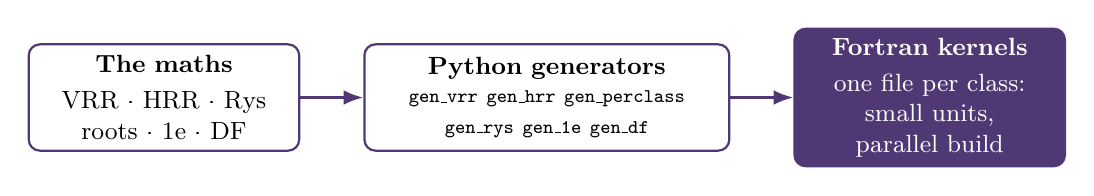
\begin{tikzpicture}[
      box/.style={draw=fortranPurple,line width=.8pt,rounded corners=4pt,fill=white,
                  minimum height=1.35cm,text width=3.2cm,align=center,font=\small},
      arr/.style={-{Latex[length=2.5mm]},line width=1pt,fortranPurple}]
    \node[box] (m) {\textbf{The maths}\\[2pt]VRR \textperiodcentered\ HRR \textperiodcentered\ Rys roots \textperiodcentered\ 1e \textperiodcentered\ DF};
    \node[box,right=.8cm of m,text width=4.4cm] (g) {\textbf{Python generators}\\[2pt]{\ttfamily\scriptsize gen\_vrr gen\_hrr gen\_perclass\\ gen\_rys gen\_1e gen\_df}};
    \node[box,right=.8cm of g,fill=fortranPurple,text=white] (k) {\textbf{Fortran kernels}\\[2pt]one file per class: small units, parallel build};
    \draw[arr] (m) -- (g);
    \draw[arr] (g) -- (k);
  \end{tikzpicture}
  \par\vspace{.8em}\raggedright
  \begin{columns}[T,onlytextwidth]
    \column{.31\textwidth}
      \begin{block}{Never edited by hand}
        A new algorithm is a generator change. CI regenerates the committed kernels and requires them byte for byte.
      \end{block}
    \column{.31\textwidth}
      \begin{block}{Rys from the HGP skeleton}
        Shared decode, screening and digestion; only the integral body differs. Under 1\,s to generate, where full HGP text at f took 6\,min and 136\,MB.
      \end{block}
    \column{.31\textwidth}
      \begin{block}{DFT the same way}
        ExchCXX functionals machine-translated to Fortran: XC on the device, no libxc. \textbf{32 run today, wB97X-V included}; the rest say what they need.
      \end{block}
  \end{columns}
  \note{Python generators emit every kernel from the maths, one file per angular-momentum class, so each compile unit stays small and the build runs in parallel. Generated code is never hand-edited, and CI checks that the committed set regenerates byte for byte. The Rys family is spliced from a skeleton of the HGP kernel, which is what made f and g reachable. DFT follows the same pattern: the functional registry is generated from ExchCXX's own definitions; 32 functionals run today, up to wB97X-V with range-separated exchange and VV10, and every other ExchCXX functional is registered with an explicit "not available: needs X" error.}
\end{frame}

% =====================================================================
\section{Performance}

\begin{frame}{Performance through d, and f now works}
  \begin{columns}[T,onlytextwidth]
    \column{.31\textwidth}
      \bignum{6.8$\times$}\par
      \textbf{faster than LibERI}\par
      \cplx{w404, 6-31G (5k basis functions); one Fock build: 22\,s vs 149\,s}
    \column{.31\textwidth}
      \bignum[fortranPurpleMid]{$\pm$10\%}\par
      \textbf{of gmshpc's CUDA C}\par
      \cplx{w172, 1e-10: 6-31G* 2.26 vs 2.37\,s; 6-31G 0.968 vs 0.887\,s}
    \column{.31\textwidth}
      \bignum{0.92$\times$}\par
      \textbf{of GPU4PySCF's time (d)}\par
      \cplx{w20, cc-pVTZ without f (1100 AOs), Fock build: 0.77 vs 0.84\,s}
  \end{columns}
  \vspace{.6em}
  \begin{columns}[T,onlytextwidth]
    \column{.52\textwidth}
      \begin{exampleblock}{Milestone: f functions}
        \begin{itemize}\setlength\itemsep{2pt}\small
          \item Every class with an f shell is one of \textbf{175 generated Rys kernels}; HGP stays at d.
          \item Matches pyscf on the first build: Fock 8e-13 (water/cc-pVTZ), 2.6e-11 (formamide/def2-TZVP); RHF to 6e-12.
          \item Roots to 9, so g is reachable. Full GPU build $\sim$32\,min on 4 cores.
        \end{itemize}
      \end{exampleblock}
    \column{.44\textwidth}
      \small
      \begin{tabular}{@{}lrr@{}}
        \toprule
        cc-pVTZ Fock, 1e-13 & Terco & GPU4PySCF \\
        \midrule
        w10, f (650 AOs)  & 0.70\,s & 0.65\,s \\
        w20, f (1300 AOs) & 2.20\,s & 1.44\,s \\
        w20, no f (1100)  & 0.77\,s & 0.84\,s \\
        \bottomrule
      \end{tabular}\par\smallskip
      \cplx{The f kernels are untuned; tuning has not started.}
  \end{columns}
  \vfill
  \src{One V100. Two-electron gradient against GPU4PySCF, 6-31G*: 0.51$\times$ its time at w20, 1.24$\times$ at w150 (8.41 vs 6.8\,s).}
  \note{All on one V100. LibERI: one Fock build of w404 in 6-31G, 22 s against 149 s. gmshpc on w172 at 1e-10: about 5\% faster in 6-31G* and about 9\% slower in 6-31G, so standard Fortran costs at most about 10\% against hand-written CUDA. GPU4PySCF 1.8.1: ahead through d. The f panel is a capability milestone, not a race: f works, in standard Fortran, and it is validated, spherical and Cartesian, CPU and GPU. The f classes alone cost Terco about 2.4 times what they cost GPU4PySCF today, and those kernels are untuned (mostly loop-form Rys). Gradient: 0.51x at w20, 0.90x at w50, 1.13x at w100, 1.24x at w150.}
\end{frame}

% =====================================================================
\section{What is new}

\begin{frame}{New: an analytic two-electron gradient}
  \vspace{-.4em}
  \begin{columns}[T,onlytextwidth]
    \column{.52\textwidth}
      {\footnotesize Rys, derivatives by raising angular momentum, D by translational invariance, RHF and UKS-ready, in pure \texttt{do concurrent}. w150 6-31G*, 1e-13:}\par
      \bignum{31.8\,s $\rightarrow$ 8.4\,s}\par
      \begin{enumerate}\setlength\itemsep{1pt}\footnotesize
        \item \textbf{Ordered compaction:} screen, then compute only survivors; ket-uniform warps 6\% $\rightarrow$ 68\%
        \item \textbf{Lane-private gradients:} no same-address FP64 atomics; (ss$|$ss) $-47\%$
        \item \textbf{Chunked heavy classes:} (pp$|$pp) 0.64 $\rightarrow$ 0.13\,s, (dp$|$pp) 1.56 $\rightarrow$ 0.33\,s
      \end{enumerate}
    \column{.44\textwidth}
      \begin{block}{Validated, not frozen}
        \footnotesize pyscf \texttt{int2e\_ip1} to 1e-12 and finite differences; no test checks Terco against its own output. A CUDA twin of the same algorithm was within 1.1--1.3$\times$: the gap left is algorithmic.
      \end{block}
      \begin{block}{Running today, and next}
        \footnotesize DFT through wB97X-V (range separation, VV10), RKS and UKS, pyscf to $\sim$3e-11; f energies; MPI and a \texttt{bind(c)} ABI.\par\smallskip
        \textbf{Next:} f tuning, f gradients, meta-GGAs, density fitting.
      \end{block}
  \end{columns}
  \begin{alertblock}{For GAMESS}
    \small GPU HF, DFT and gradients in standard Fortran its developers can read and extend: no CUDA, no C++.
  \end{alertblock}
  \note{The genuinely new part is the analytic two-electron gradient via Rys quadrature in pure do concurrent. Development took w150 6-31G* at 1e-13 from 31.8 s to 8.4 s (3.8x): ordered survivor compaction in runs of 32 so warps stay ket-uniform; 32 lane-private copies of the gradient to stop same-address FP64 atomic serialisation ((ss|ss) -47\%, (ps|ss) -33\%); and a chunked compact pass for heavy classes. A same-algorithm CUDA twin came within 1.1-1.3x, so what separates Terco from GPU4PySCF is algorithm, not a language tax. Already running: DFT up to wB97X-V, RKS and UKS, validated against pyscf to about 3e-11, 32 runnable functionals; f energies, validated. Capability first, tuning later. The pitch: this is the avenue for GAMESS on GPUs.}
\end{frame}

\begin{frame}{Gradient: ordered survivor compaction}{Screen first, then compute only survivors, in an order that keeps warps uniform}
  \centering
  \begin{tikzpicture}[font=\footnotesize,
      lane/.style={minimum width=.26cm,minimum height=.36cm,inner sep=0pt,draw=white,line width=.3pt},
      arr/.style={-{Latex[length=2mm]},line width=.8pt,fortranPurple}]
    % pattern of survivors in 32 work items (schematic)
    \def\pat{1,0,0,1,1,0,0,0,1,0,1,1,0,0,0,1,0,0,1,0,1,0,0,0,1,1,0,0,1,0,0,1}
    \node[anchor=west,font=\footnotesize\bfseries] at (0,2.95) {Fused: one warp, 32 work items};
    \foreach \v [count=\i from 0] in \pat {
      \ifnum\v=1 \node[lane,fill=fortranPurple] at (\i*.27+.13,2.45) {};
      \else      \node[lane,fill=cookieLine]    at (\i*.27+.13,2.45) {}; \fi }
    \node[anchor=west,cookieMuted,font=\scriptsize,text width=8.3cm] at (0,1.95)
      {every lane screens, then the survivors run the integral body while the rest idle: divergence};
    \draw[arr] (4.3,1.7) -- (4.3,1.3);
    \node[anchor=west,font=\footnotesize\bfseries] at (0,1.05) {Screen pass: chunks of 32 (one warp), one atomic capture per chunk};
    \foreach \v [count=\i from 0] in \pat {
      \ifnum\v=1 \node[lane,fill=fortranPurple] at (\i*.27+.13,.55) {};
      \else      \node[lane,fill=cookieLine]    at (\i*.27+.13,.55) {}; \fi }
    \draw[arr] (4.3,.3) -- (4.3,-.1);
    \node[anchor=west,font=\footnotesize\bfseries] at (0,-.35) {Compact pass: dense survivor list, in item order};
    \foreach \i in {0,...,12} { \node[lane,fill=fortranPurple] at (\i*.27+.13,-.85) {}; }
    \foreach \i in {13,...,31} { \node[lane,fill=fortranPurpleMid!45] at (\i*.27+.13,-.85) {}; }
    \node[anchor=west,cookieMuted,font=\scriptsize,text width=8.3cm] at (0,-1.38)
      {decode is bra-fastest, so neighbours share a ket pair; the next chunk's survivors fill the warp};
    % right: lane-private gradients
    \begin{scope}[xshift=9.2cm]
      \node[anchor=west,font=\footnotesize\bfseries] at (0,2.95) {Lane-private gradients};
      \foreach \c in {0,...,5} {
        \node[draw=fortranPurple,fill=fortranPurple!10,minimum width=.48cm,minimum height=.9cm,
              font=\tiny] (g\c) at (\c*.56+.25,2.0) {$g_{\c}$};
      }
      \node[font=\scriptsize,anchor=west] at (3.3,2.0) {\dots\ $g_{31}$};
      \node[anchor=west,font=\scriptsize,text width=4.4cm] at (0,1.05)
        {survivor $i$ adds into copy $\mathrm{mod}(i{-}1,32){+}1$: no same-address FP64 atomics; summed once at the end};
      \node[anchor=west,font=\footnotesize\bfseries] at (0,-.1) {Measured, w150 6-31G*};
      \node[anchor=west,font=\scriptsize,text width=4.4cm] at (0,-.85)
        {(ps|ss): fused 3.97\,s $\rightarrow$ per-item append 3.31\,s $\rightarrow$ chunks of 32 2.15\,s\\
         (ss|ss)+(ps|ss): 1 copy 3.11\,s $\rightarrow$ 32 copies 1.91\,s};
    \end{scope}
  \end{tikzpicture}
  \vfill
  {\scriptsize\color{cookieMuted} Survivor pattern schematic. Both passes are sliced from the same generated text: nothing in the integral body is retyped.}
  \note{The first optimisation on the gradient, drawn. The fused kernel screens and computes in the same warp, so a warp in which only a few of 32 work items survive runs the full Rys body with most lanes idle; ket-uniform warps were 6 percent. The screen pass walks 32 consecutive work items per do concurrent iteration, one warp's worth, and appends the chunk's survivors with one atomic capture sized to its own count, in item order. Because the decode is bra-fastest, consecutive survivors share a ket pair, so the compact pass, running over the dense list, sees warps that are 68 percent ket-uniform. Measured on (ps|ss), w150 6-31G* at 1e-13: 3.97 s fused, 3.31 s with a per-item append, 2.15 s with chunks of 32; 64, 128 and 256 were slower. The second step gives each lane its own copy of the gradient, 32 copies of 3 x natm, so lanes never fight over the same address; that took (ss|ss)+(ps|ss) from 3.11 to 1.91 s. Both passes are cut out of the same generated kernel text.}
\end{frame}

\end{document}
